\section{Graph Convolutional Network (GCN)}
\glsreset{GCN}
Graphs are commonly used structures representing complex systems, including social networks, biological networks, and transportation systems \autocite{scarselli2008graph}. They consist of nodes and edges, representing the entities and relationships between them. Despite their widespread use, graphs pose unique challenges in machine learning due to their irregular structure, which makes it difficult to apply conventional learning techniques that rely on fixed-size inputs and Euclidean data representations \autocite{battaglia2018relational}.

\Gls{GNN} has emerged as a solution to these challenges, generalising deep learning techniques to graph-structured data \autocite{gori2005new}. Among \glspl{GNN}, \glspl{GCN} have become particularly popular owing to their ability to perform localised and efficient convolutions on graph data \autocite{DBLP:journals/corr/KipfW16}. \glspl{GCN} extend the concept of convolution from grid-like structures, such as images, to irregular graph structures, enabling the extraction of meaningful features from graph data while preserving their spatial relationships \autocite{bronstein2017geometric}. 

\subsection{Graph Convolutions}
The core of \glspl{GCN} lies in the graph convolution operation, which aims to aggregate local information from neighbouring nodes to generate a new representation for each node. The main idea is to perform a weighted sum of the feature vectors of a node and its neighbours, where the weights are determined by the edge weights or some measure of node similarity. For instance, the feature vector of a node (a person) in a social network graph could include elements such as age, number of friends, job category, etc., that offer unique details about that node.  This aggregation scheme allows \glspl{GCN} to learn node representations that effectively capture the local graph structure. The \cref{eq:kiph}, found in \autocite{DBLP:journals/corr/KipfW16}, shows how the graph convolution operation is mathematically described.

\begin{equation} 
    \bm{H}^{l+1} = \sigma(\bm{\hat{D}}^{-\frac{1}{2}} \bm{A} \bm{\hat{D}}^{-\frac{1}{2}} \bm{H}^{l} \bm{W}^{l} )
    \label{eq:kiph}
\end{equation}


The components in \cref{eq:kiph} are defined as follows \autocite{DBLP:journals/corr/KipfW16}:

$H^{(l+1)}$ stands for the updated node representations (features) at layer $(l+1)$, while $H^{(l)}$ indicates the node features at layer $l$. $H^{(0)}$ is the input feature matrix for the first layer. The graph's adjacency matrix, represented by $A$, is modified to incorporate self-connections. This is achieved by adding a diagonal matrix with ones to the original adjacency matrix $A$, ensuring that the node's features are considered during the aggregation process.

The degree matrix, denoted by $\hat{D}$, corresponds to the modified adjacency matrix $\hat{A}$. It is a diagonal matrix wherein each diagonal entry signifies the degree (number of connections) of the corresponding node. The learnable weight matrix at layer $l$ is represented by $W^{(l)}$ and is employed to transform the node features at each layer linearly.

Lastly, the activation function $\sigma$ introduces non-linearity to the model. Typical choices for activation functions are ReLU, sigmoid, and tanh.

In the graph shown in \cref{fig:graph}, the nodes represent entities, and the lines between nodes represent the relationships between these entities. Here, we have four nodes: A, B, C, and D, and the connection between them. 

The adjacency matrices (\cref{eq:matrix} and \cref{eq:matrix2}) are mathematical representations of the graph. In the matrices, the value at the intersection of a row and a column represents the presence (1) or absence (0) between the nodes.

\begin{figure}[h!]
    \begin{minipage}{0.30\textwidth}
    \centering
    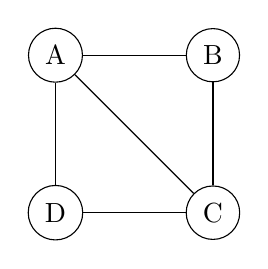
\begin{tikzpicture}[every node/.style={circle, draw}]
    \node (A) at (0,0) {A};
    \node (B) at (2,0) {B};
    \node (C) at (2,-2) {C};
    \node (D) at (0,-2) {D};
    \draw (A) -- (B) -- (C) -- (D) -- (A);
    \draw (A) -- (C);
    \end{tikzpicture}
    \caption{Graph with 4 nodes}
    \label{fig:graph}
    \end{minipage}
    \hfill
    \begin{minipage}{0.30\textwidth}
    \centering
    \[
    A = \begin{bmatrix}
    0 & 1 & 1 & 1 \\
    1 & 0 & 1 & 0 \\
    1 & 1 & 0 & 1 \\
    1 & 0 & 1 & 0 \\
    \end{bmatrix}
    \]

    \captionof{figure}{Adjacency matrix corresponding to the graph without self-connections}
    \label{eq:matrix}
    \end{minipage}
    \hfill
    \begin{minipage}{0.30\textwidth}
    \centering
    \[
    A = \begin{bmatrix}
    1 & 1 & 1 & 1 \\
    1 & 1 & 1 & 0 \\
    1 & 1 & 1 & 1 \\
    1 & 0 & 1 & 1 \\
    \end{bmatrix}
    \]

    \captionof{figure}{Adjacency matrix corresponding to the graph with self-connections}
    \label{eq:matrix2}
    \end{minipage}
\end{figure}





